\section{Result}\label{sec:result}

This section presents the results of the models described in Section~\ref{sec:methology}.
The results are presented in the form of graphs and tables.
The graphs are plotted using the \texttt{seaborn}~\cite{seaborn} and \texttt{matplotlib}~\cite{matplot} library.
Each evaluation includes the following graphs and tables:
\begin{itemize}
    \item \textbf{Accuracy and loss graph}:
          The accuracy and loss graph shows the accuracy and loss of the model during training and validation
          using the \texttt{accuracy} and \texttt{loss} metrics provided by Keras.
    \item \textbf{Performance metrics}:
          The performance metrics table shows the performance metrics of the model on the held back test set calculated using the \texttt{classification\_report} function from \texttt{sklearn}~\cite{scikit-learn}.
          Its metrics include precision, recall, f1-score, and support, as well as the overall accuracy of the model.
    \item \textbf{Confusion matrix}:
          The confusion matrix shows the number of true positives, false positives, true negatives,
    and false negatives calculated using the \texttt{confusion\_matrix} function from \texttt{sklearn}~\cite{scikit-learn}.
          The labels 0--5 correspond to the classes \texttt{WALKING}, \texttt{WALKING\_UPSTAIRS},
    \texttt{WALKING\_DOWNSTAIRS}, \texttt{SITTING}, \texttt{STANDING},
    and \texttt{LAYING}, respectively.
\end{itemize}

\subsection{Feedforward Neural Network}\label{subsec:feedforward-neural-network}

\subsubsection{Simple Feedforward Neural Network}

Figure~\ref{fig:ffnn-simple-accuracy-loss-graph} shows the accuracy and loss graph for the simple feedforward neural network.
The graph shows that the training accuracy started at around 0.85 and increased to around 0.98 after 100 epochs,
which is a steady increase matching the training loss.
The validation accuracy started at around 0.95
and ended at about the same value after fluctuating between 0.9 and 0.975,
with one spike at around 0.825.
That the validation accuracy started so high indicates that the problem is not very difficult,
however, the fluctuation indicates that the model is not very stable and potentially overfitting.

This is further supported by the performance metrics in Figure~\ref{fig:ffnn-simple-performance-metrics}
which evaluate the model on the held back test set.
The metrics indicate that the model is good at identifying the classes \texttt{WALKING},
\texttt{WALKING\_UPSTAIRS}, \texttt{WALKING\_DOWNSTAIRS},
and \texttt{LAYING}, but struggles at identifying \texttt{SITTING} and \texttt{STANDING}.
The overall accuracy of the model is 0.89, which is pretty good for a simple model that was not tuned.

Looking at the confusion matrix in Figure~\ref{fig:ffnn-simple-confusion-matrix},
we can see that it often confuses \texttt{STANDING} with \texttt{SITTING}.
Which explains why performance metrics for these two classes are lower than the others.

\begin{figure}[ht]
    \centering
    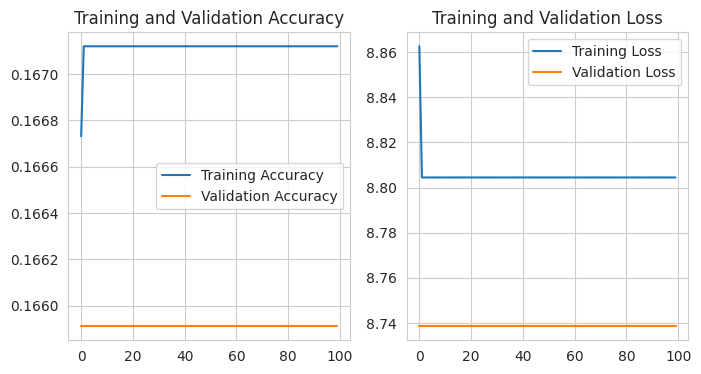
\includegraphics[width=0.85\textwidth]{./img/ffnn/simple/accuracy-loss-graph}
    \caption{Accuracy and loss graph for the simple feedforward neural network.}
    \label{fig:ffnn-simple-accuracy-loss-graph}
\end{figure}

\begin{figure}[ht]
    \centering
    \begin{minipage}{0.45\textwidth}
        \centering
        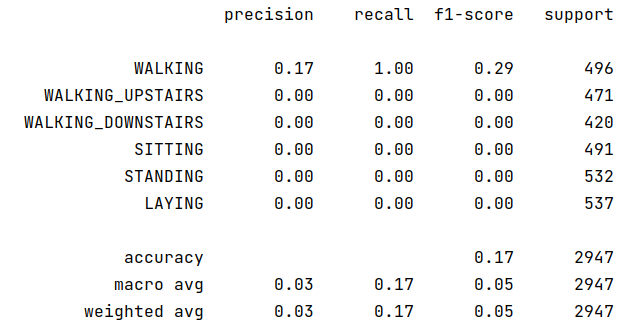
\includegraphics[width=\textwidth]{./img/ffnn/simple/performance-metrics}
        \caption{Performance metrics for the simple feedforward neural network.}
        \label{fig:ffnn-simple-performance-metrics}
    \end{minipage}\hfill
    \begin{minipage}{0.45\textwidth}
        \centering
        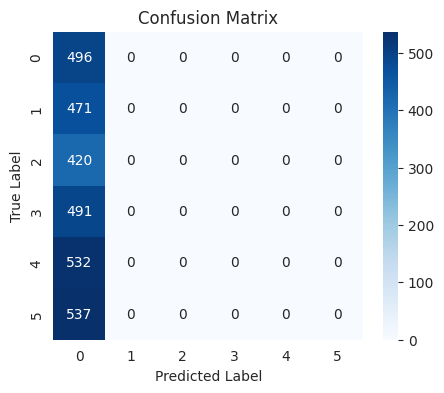
\includegraphics[width=\textwidth]{./img/ffnn/simple/confusion-matrix}
        \caption{ Confusion matrix for the simple feedforward neural network.}
        \label{fig:ffnn-simple-confusion-matrix}
    \end{minipage}
\end{figure}

\subsubsection{Tuned Complex Feedforward Neural Network}

After tuning the hyperparameters of the feedforward neural network,
we end up with the architecture shown in Figure~\ref{fig:fnn-best-params}.
Which consists of 2 dense layers with 384 and 640 neurons, respectively, and a dropout layer with a dropout rate of 0.1,
followed by 6 dense layers with 32 neurons each.
Making it more complex than the simple feedforward neural network.

This increased complexity seems to allow the model to learn more about the data,
as shown in Figure~\ref{fig:ffnn-tuned-accuracy-loss-graph}.
The training accuracy starts at over 0.99 and hits 1.0 several times during training,
while the validation accuracy starts and ends at around 0.98.
This indicates that the model is probably overfitting,
but the validation accuracy is still higher than the training accuracy of the simple feedforward neural network,
which indicates that the model is more stable.
While the fluctuation might seem more intense than in the simple feedforward neural network,
it is important to note that the y-axis is scaled differently,
and the fluctuation is actually smaller.

The performance metrics in Figure~\ref{fig:ffnn-tuned-performance-metrics} also show
that the model got
a lot better at identifying \texttt{SITTING} and \texttt{STANDING} compared to the simple feedforward neural network.
The overall accuracy of the model is 0.94, which is a good improvement over the simple feedforward neural network.

Looking at the confusion matrix in Figure~\ref{fig:ffnn-tuned-confusion-matrix},
we can see that it still sometimes confuses \texttt{STANDING} and \texttt{SITTING},
but not as often as the simple feedforward neural network.

Overall, the model seems to be doing a good job at identifying the classes, and it also seems to generalize better than the simple feedforward neural network.

\begin{figure}[ht]
    \centering
    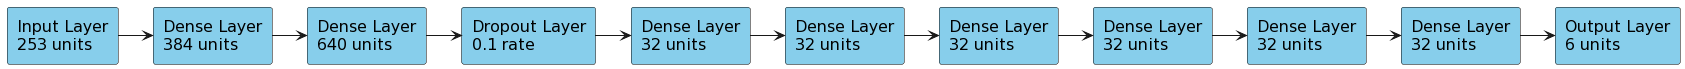
\includegraphics[width=\textwidth]{./img/ffnn/tuned/fnn-best-params}
    \caption{Visualization of tuned feedforward neural network architecture}
    \label{fig:fnn-best-params}
\end{figure}

\begin{figure}[ht]
    \centering
    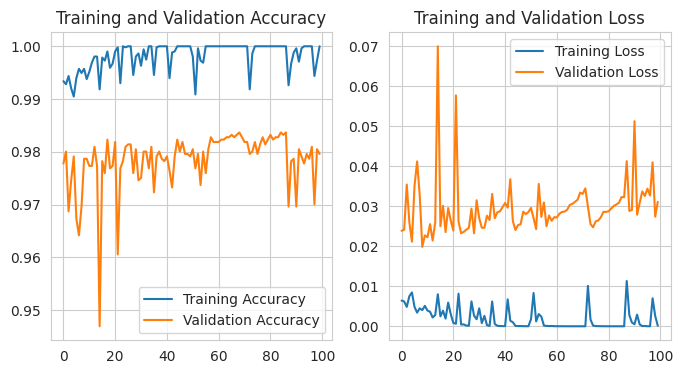
\includegraphics[width=0.85\textwidth]{./img/ffnn/tuned/accuracy-loss-graph}
    \caption{Accuracy and loss graph for the tuned feedforward neural network.}
    \label{fig:ffnn-tuned-accuracy-loss-graph}
\end{figure}

\begin{figure}[ht]
    \centering
    \begin{minipage}{0.45\textwidth}
        \centering
        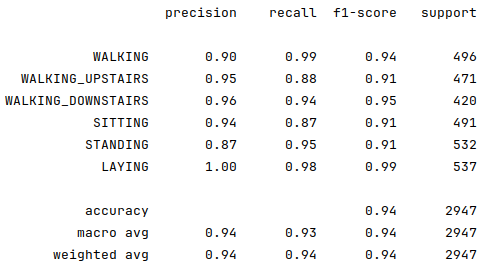
\includegraphics[width=\textwidth]{./img/ffnn/tuned/performance-metrics}
        \caption{Performance metrics for the tuned feedforward neural network.}
        \label{fig:ffnn-tuned-performance-metrics}
    \end{minipage}\hfill
    \begin{minipage}{0.45\textwidth}
        \centering
        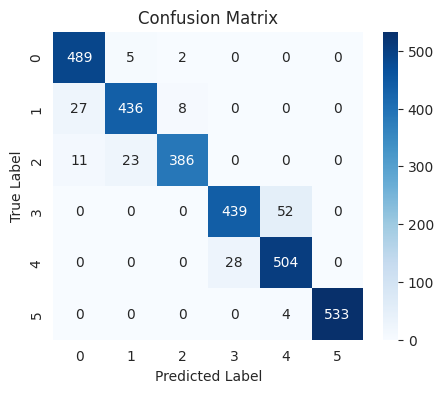
\includegraphics[width=\textwidth]{./img/ffnn/tuned/confusion-matrix}
        \caption{Confusion matrix for the tuned feedforward neural network.}
        \label{fig:ffnn-tuned-confusion-matrix}
    \end{minipage}
\end{figure}

\subsection{Convolutional Neural Network}\label{subsec:convolutional-neural-network}

\subsubsection{Simple Convolutional Neural Network}

Figure~\ref{fig:cnn-simple-accuracy-loss-graph} shows the accuracy and loss graph for the simple convolutional neural network.
It has a steady increase in training and validation accuracy, and a steady decrease in training and validation loss.
It also seems to be pretty stable as it does not fluctuate much, however this might be because the y-axis is scaled differently, as it starts at 0.4.
The starting accuracies are also more in line with what you would normally expect from a model that has not been fitted to the data.
What is really curious is that the validation accuracy is consistently higher than the training accuracy, which is not something you would normally expect and might indicate that the model is underfitting.

Looking at the performance metrics in Figure~\ref{fig:cnn-simple-performance-metrics}, the model seems to be performing slightly worse than the simple feedforward neural network, with an overall accuracy of 0.88.
Interestingly it seems to struggle with categorizing \texttt{WALKING} and \texttt{WALKING\_UPSTAIRS}.

The confusion matrix in Figure~\ref{fig:cnn-simple-confusion-matrix} that the mistakes it makes are more distributed than the simple feedforward neural network.
This could mean that the error the model makes has less bias than the simple feedforward neural network.

Overall, the model still performs decently, but it does not seem to be an improvement over the simple feedforward neural network.

\begin{figure}[ht]
    \centering
    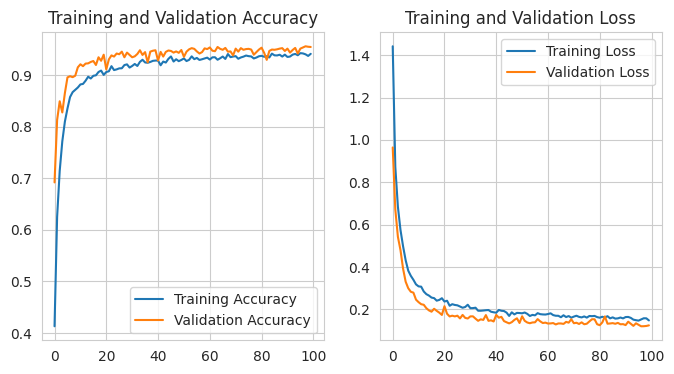
\includegraphics[width=0.85\textwidth]{./img/cnn/simple/accuracy-loss-graph}
    \caption{Accuracy and loss graph for the simple convolutional neural network.}
    \label{fig:cnn-simple-accuracy-loss-graph}
\end{figure}

\begin{figure}[ht]
    \centering
    \begin{minipage}{0.45\textwidth}
        \centering
        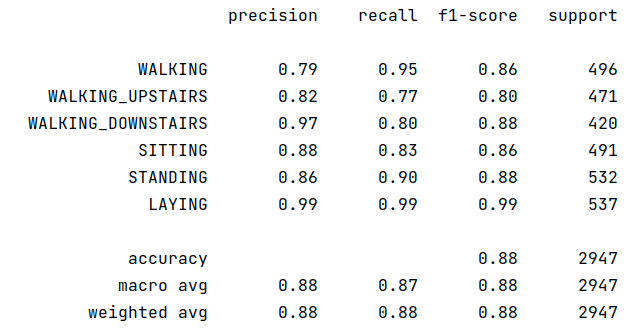
\includegraphics[width=\textwidth]{./img/cnn/simple/performance-metrics}
        \caption{Performance metrics for the simple convolutional neural network.}
        \label{fig:cnn-simple-performance-metrics}
    \end{minipage}\hfill
    \begin{minipage}{0.45\textwidth}
        \centering
        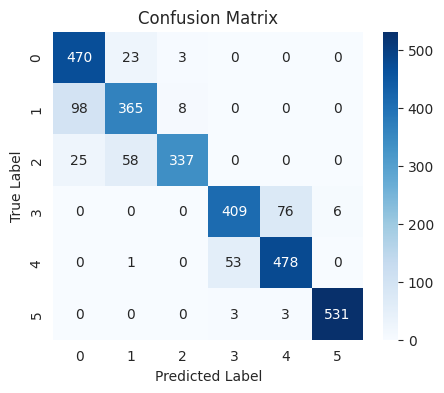
\includegraphics[width=\textwidth]{./img/cnn/simple/confusion-matrix}
        \caption{Confusion matrix for the simple convolutional neural network.}
        \label{fig:cnn-simple-confusion-matrix}
    \end{minipage}
\end{figure}

\subsubsection{Tuned Convolutional Neural Network}

After tuning the hyperparameters of the convolutional neural network,
we end up with the architecture shown in Figure~\ref{fig:cnn-best-params}.
In contrast to the untuned convolutional neural network, the first convolutional layer has 112 filters instead of 25, the second convolutional layer has 64 filters instead of 32 and the dropout rate is 0.0 instead of 0.2.

As Figure~\ref{fig:cnn-tuned-accuracy-loss-graph} shows, this small change allows for the training accuracy to reach 1.0, while the validation accuracy fluctuates mostly between 0.98 and 0.97.
This indicates that the model is overfitting the training data.

The performance metrics in Figure~\ref{fig:cnn-tuned-performance-metrics} show that the model is performing better than the simple convolutional neural network, with an overall accuracy of 0.94.
And having pretty good scores on the metrics for all the classes.

The confusion matrix in Figure~\ref{fig:cnn-tuned-confusion-matrix} shows that the model is still making some mistakes, but it is doing a pretty good job at classifying the activities.

\begin{figure}[ht]
    \centering
    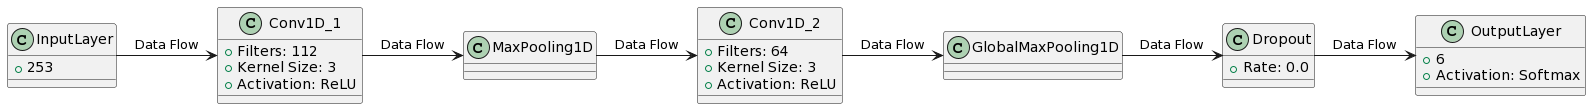
\includegraphics[width=\textwidth]{./img/cnn/tuned/cnn-best-params}
    \caption{Visualization of tuned convolutional neural network architecture}
    \label{fig:cnn-best-params}
\end{figure}

\begin{figure}[ht]
    \centering
    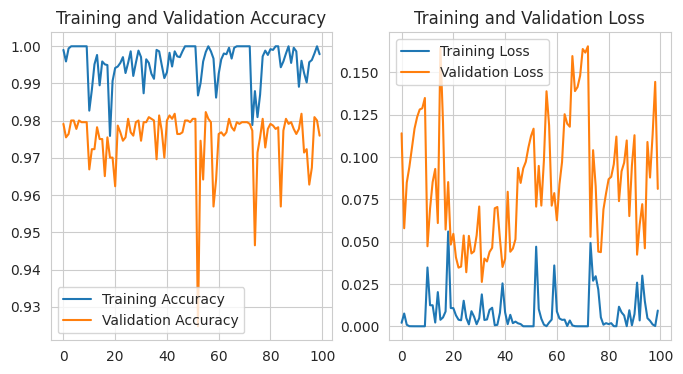
\includegraphics[width=0.85\textwidth]{./img/cnn/tuned/accuracy-loss-graph}
    \caption{Accuracy and loss graph for the tuned convolutional neural network.}
    \label{fig:cnn-tuned-accuracy-loss-graph}
\end{figure}

\begin{figure}[ht]
    \centering
    \begin{minipage}{0.45\textwidth}
        \centering
        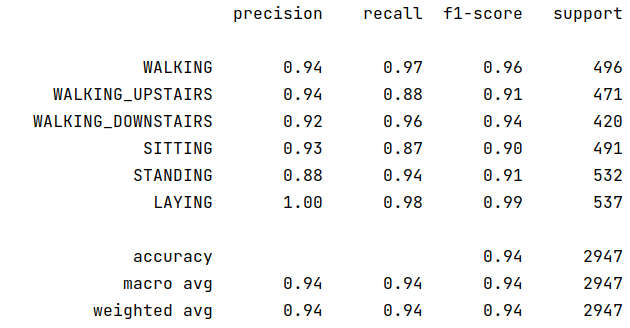
\includegraphics[width=\textwidth]{./img/cnn/tuned/performance-metrics}
        \caption{Performance metrics for the tuned convolutional neural network.}
        \label{fig:cnn-tuned-performance-metrics}
    \end{minipage}\hfill
    \begin{minipage}{0.45\textwidth}
        \centering
        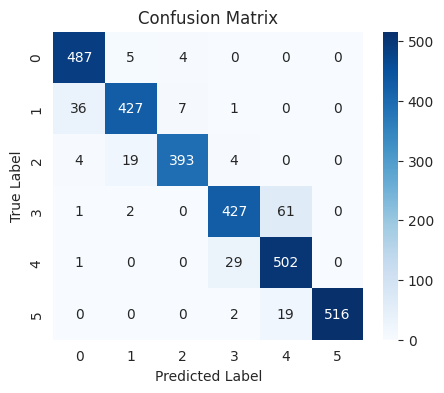
\includegraphics[width=\textwidth]{./img/cnn/tuned/confusion-matrix}
        \caption{Confusion matrix for the tuned convolutional neural network.}
        \label{fig:cnn-tuned-confusion-matrix}
    \end{minipage}
\end{figure}


\subsection{Long Short-Term Memory}\label{subsec:long-short-term-memory}

Looking at the accuracy and loss graph in Figure~\ref{fig:lstm-accuracy-loss-graph}, the lstm seems to be able to learn the data.
However, the performance metrics in Figure~\ref{fig:lstm-performance-metrics} show that the model performs really bad on the test set, with an overall accuracy of 0.33.

The confusion matrix in Figure~\ref{fig:lstm-confusion-matrix} shows that it classifies pretty much everything as \texttt{WALKING\_DOWNSTAIRS}.

We could not figure out why the models had such bad performance.
The training and validation accuracy and loss graphs look fine, and the model seems to be able to learn the data.
The only guess we have, is that we feed the time series data into the model in the wrong format.
However, we decided not to spend more time on this and we already had models that performed well.

\begin{figure}[ht]
    \centering
    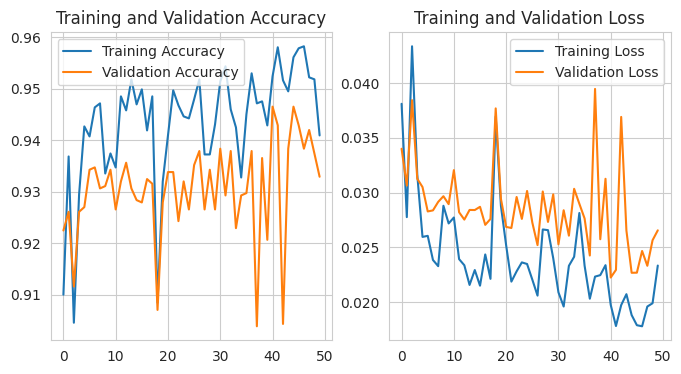
\includegraphics[width=0.85\textwidth]{./img/lstm/accuracy-loss-graph}
    \caption{Accuracy and loss graph for the long short-term memory model.}
    \label{fig:lstm-accuracy-loss-graph}
\end{figure}

\begin{figure}[ht]
    \centering
    \begin{minipage}{0.45\textwidth}
        \centering
        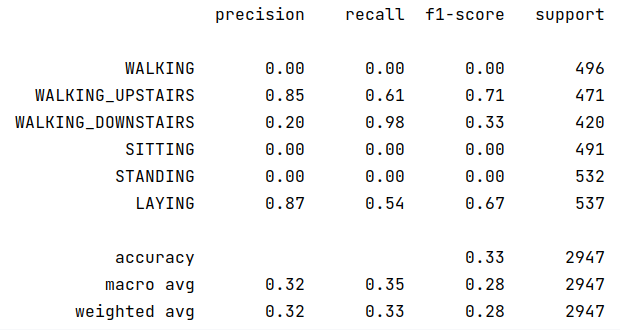
\includegraphics[width=\textwidth]{./img/lstm/performance-metrics}
        \caption{Performance metrics for the long short-term memory model.}
        \label{fig:lstm-performance-metrics}
    \end{minipage}\hfill
    \begin{minipage}{0.45\textwidth}
        \centering
        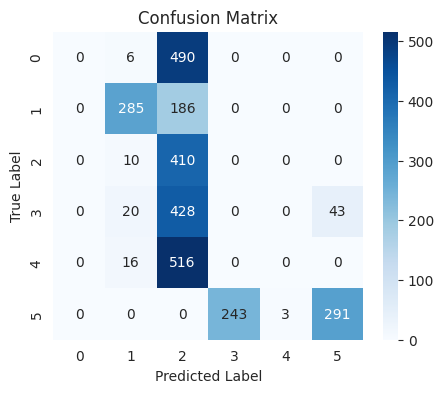
\includegraphics[width=\textwidth]{./img/lstm/confusion-matrix}
        \caption{Confusion matrix for the long short-term memory model.}
        \label{fig:lstm-confusion-matrix}
    \end{minipage}
\end{figure}

\subsection{Transformer}\label{subsec:transformer}

Again, looking at the accuracy and loss graph in Figure~\ref{fig:transformer-accuracy-loss-graph}, the transformer seems to be able to learn the data.
However, the performance metrics in Figure~\ref{fig:transformer-performance-metrics} show that the model performs really bad on the test set, with an overall accuracy of around 0.17, which is about as good as guessing.
The confusion matrix in Figure~\ref{fig:transformer-confusion-matrix} shows that it classifies almost everything as \texttt{WALKING\_UPSTAIRS}.

We think that we have the same problem as with the lstm model.

\begin{figure}[ht]
    \centering
    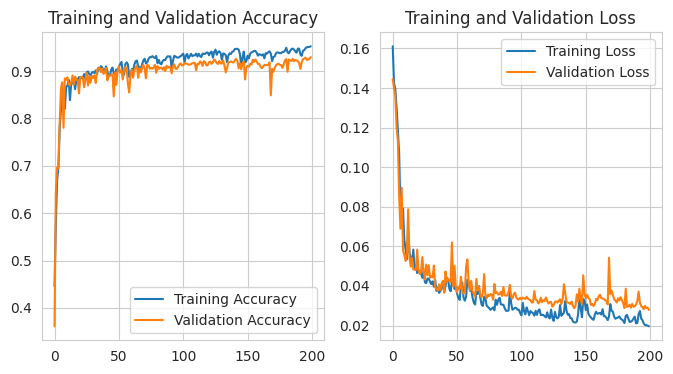
\includegraphics[width=0.85\textwidth]{./img/transformer/accuracy-loss-graph}
    \caption{Accuracy and loss graph for the transformer model.}
    \label{fig:transformer-accuracy-loss-graph}
\end{figure}

\begin{figure}[ht]
    \centering
    \begin{minipage}{0.45\textwidth}
        \centering
        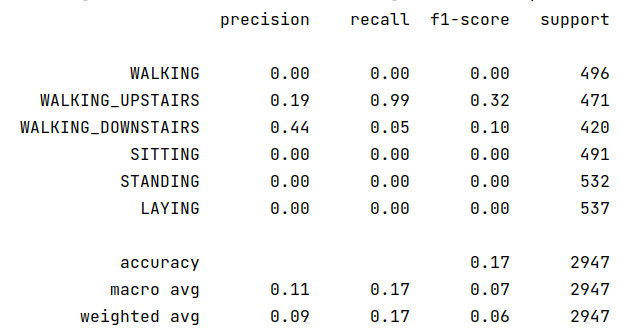
\includegraphics[width=\textwidth]{./img/transformer/performance-metrics}
        \caption{Performance metrics for the transformer model.}
        \label{fig:transformer-performance-metrics}
    \end{minipage}\hfill
    \begin{minipage}{0.45\textwidth}
        \centering
        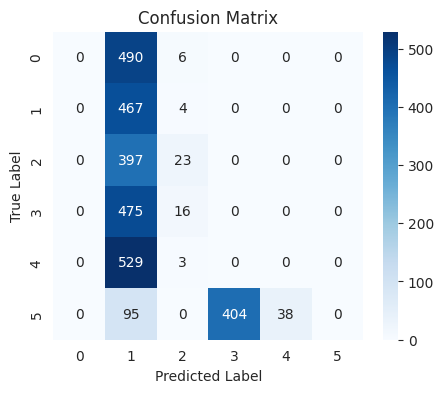
\includegraphics[width=\textwidth]{./img/transformer/confusion-matrix}
        \caption{Confusion matrix for the transformer model.}
        \label{fig:transformer-confusion-matrix}
    \end{minipage}
\end{figure}

